\chapter{Revisão Teórica}\label{cap2_revisao}
{ Alguns conceitos são essenciais para compreender o projeto proposto, sua
    implementação e seus resultados. Esse capítulo abordará o que é arquitetura
    e organização de computadores, tratará brevemente sobre as arquiteturas mais
    conhecidas e se aprofundará na especificação da arquitetura \textit{RISC-V}.
    Além disso, serão expostos os conceitos de síntese de \textit{hardware} e
    do funcionamento das \textit{FPGAs}, em especial o modelo que será utilizado
    para desenvolver o trabalho.
    Por fim, o ``estado da arte'' da arquitetura \textit{RISC-V} será discutido.
}

\section{Arquitetura de Computadores}
{ Para nos comunicarmos, necessitamos de uma linguagem, e no caso dos
    brasileiros, essa linguagem é o português. Como toda linguagem, o português
    possui sua gramática e dicionário que lhe dá estrutura e sentido. Línguas
    humanas como o português, inglês e espanhol são chamadas de linguagens
    naturais, e evoluíram naturalmente a partir do uso e
    repetição.~\cite{lyons1991natural}
}

{ Por causa da excelente capacidade de interpretação e adaptação da mente
    humana, somos capazes de criar e entender novos dialetos que não seguem as
    regras formais das linguagens naturais que conhecemos. Porém, fora da
    comunicação casual é importante e às vezes obrigatório que nos expressemos
    sem ambiguidade. Línguas artificiais como a notação matemática e linguagens
    de programação possuem semântica e sintaxe mais rígidas para garantir que
    a mensagem transmitida seja interpretada da maneira correta. Sem essa
    rigidez, os computadores de hoje não seriam capazes de entender nossos
    comandos.
}

{ Para a comunicação com o processador de um computador, utilizamos mensagens
    chamadas de instruções, e o conjunto dessas instruções é chamado de
    Arquitetura do Conjunto de Instruções (\textit{ISA}). Um processador só é
    capaz de entender as mensagens que obedecem as regras semânticas e
    sintáticas de sua \textit{ISA}, e qualquer instrução que fuja das suas
    regras causará um erro de execução ou realizará uma tarefa diferente da
    pretendida. A linguagem de máquina é considerada de baixo nível pois
    apresenta pouca ou nenhuma abstração em relação à arquitetura.
}

{ As instruções são passadas para o processador na forma de código de máquina,
    sequências de dígitos binários que correspondem aos níveis lógicos do
    circuito. Para melhorar o entendimento do código e facilitar seu
    desenvolvimento, uma outra representação é utilizada, o \textit{assembly}.
    Um código \textit{assembly} é transformado em código de máquina por um
    programa montador (\textit{assembler}), e o processo inverso é realizado
    por um \textit{disassembler}. As linguagens \textit{assembly}, dependendo do
    \textit{assembler} utilizado, permitem o uso de \textit{macros} de substituição
    e pseudo-instruções (determinadas instruções inexistentes na \textit{ISA}
    que são expandidas em instruções válidas pelo montador) e são totalmente
    dependentes da arquitetura do processador, o que normalmente impede que o
    mesmo código binário executável funcione em arquiteturas diferentes.
}

{ A Figura~\ref{fig:cpu_abstraction} é uma representação simplificada de um
    processador. A unidade de controle lê uma instrução da memória e a
    decodifica; o circuito de lógica combinacional lê os dados dos
    registradores, entrada e memória conforme necessário, executa a instrução
    decodificada e escreve no banco de registradores, na memória de dados ou
    na saída se for preciso; a unidade de controle lê uma nova instrução e o
    ciclo se repete até o fim do programa. A posição de memória da instrução
    que está sendo executada fica armazenada em um registrador especial chamado
    de Contador de Programa (\textit{PC}). Algumas instruções modificam o
    \textit{PC} condicionalmente ou diretamente, criando a estrutura para
    saltos, laços e chamada/retorno de funções.
}

\begin{figure}[H]
\centering
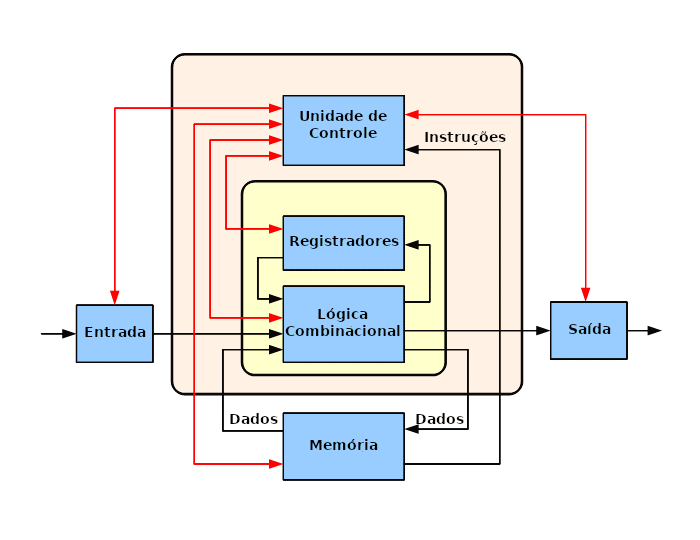
\includegraphics[width=.75\linewidth]
    {../images/ABasicComputer.png}
    \caption[Abstração da arquitetura de um computador]
    {Abstração da arquitetura de um
        computador. Fonte:~\cite{wikimedia2015basiccpu}}\label{fig:cpu_abstraction}
\end{figure}

    \subsection{Arquiteturas \textit{RISC} e \textit{CISC}}
    { Historicamente, as arquiteturas são divididas em \textit{ISAs} \textit{RISC}
        (\textit{Reduced Instruction Set Computer}) e \textit{CISC}
        (\textit{Complex Instruction Set Computer}).  Na atualidade, a principal
        diferença entre elas é que as \textit{ISAs RISC} acessam a memória por
        instruções de \textit{load/store}, enquanto as \textit{CISC} podem acessar
        a memória diretamente em uma instrução de operação lógica ou
        aritmética.~\cite{risc_cisc_wars}
    }

    { Algumas arquiteturas \textit{RISC} notáveis são a \textit{RISC-V}, objeto de
        estudo desse trabalho, a \textit{ARM} e a \textit{MIPS}. Quanto às
        \textit{CISC}, a \textit{x86} e sua extensão de 64 \textit{bits}, a
        \textit{AMD64}, são as mais conhecidas e amplamente utilizadas.
    }

    \subsection{Arquitetura MIPS}
    { Durante seus 36 anos de existência, a \textit{ISA MIPS} (\textit{Microprocessor
        without Interlocked Pipelined Stages}) teve diversas versões produzidas,
        atendendo às demandas de diversos segmentos do mercado. Usado em
        supercomputadores na década de 90 e nos famosos \textit{videogames
        Nintendo 64, PlayStation, PlayStation 2 e PlayStation Portable}, a
        arquitetura atendia a vários segmentos do mercado.
    }

    { A \textit{MIPS32}, uma de suas versões lançada em 1999~\cite{mips32_1999},
        é amplamente utilizada no meio acadêmico, utilizando livros como as
        diversas edições do \textit{Computer Organization and
        Design}~\cite{patterson2014computer} e o clássico
        \textit{See MIPS run}~\cite{sweetman1999see} como livros-texto das
        disciplinas de arquitetura de computadores.
    }

    { Na última década, o uso de processadores \textit{MIPS} têm se limitado a
        sistemas automotivos e roteadores de \textit{internet}~\cite{mips_uses_wiki},
        e a empresa detentora dos direitos da arquitetura anunciou o fim do
        desenvolvimento de novas iterações.~\cite{wave_comp_bankrupt}
    }

    \subsection{Arquitetura ARM}
    { A arquitetura \textit{ARM} (\textit{Advanced RISC Machines}) é considerada
        extremamente eficiente no consumo de energia e possui boa dissipação de
        calor sem comprometer seu desempenho~\cite{arm_facts1988}, e com isso é
        predominante no mercado de \textit{smartphones}~\cite{arm_milestone}.
        Presente também nos \textit{videogames Nintendo 3DS e Nintendo Switch},
        nos \textit{Single Board Computers} (\textit{SBCs}) \textit{Raspberry Pi},
        entre outros dispositivos, a arquitetura tem enorme força em aplicações
        embarcadas.
    }

    { Porém, isso não a impede de atender a outros setores do mercado. Atualmente,
        o supercomputador mais potente do mundo utiliza a arquitetura
        \textit{ARM}.~\cite{arm_super} A \textit{Apple} recentemente lançou seus
        primeiros \textit{notebooks} e \textit{desktops} com seu processador
        \textit{Apple M1}, considerado hoje o processador de computadores pessoais
        com maior eficiência por \textit{watt}.~\cite{arm_m1} O serviço de
        computação em nuvem \textit{Amazon Web Services} (\textit{AWS})
        também oferece máquinas equipadas com seu processador \textit{AWS Graviton}
        para computação geral.
    }

    { A empresa \textit{ARM} opera licenciando o uso do seu conjunto de instruções
        e de projetos de implementação, mas não produz \textit{chips}. A manufatura
        do processador fica a cargo da empresa licenciante, como a \textit{Qualcomm},
        \textit{NXP}, \textit{Samsung} e \textit{Apple}.
    }

    { Por ser uma das arquiteturas prevalentes da atualidade, a \textit{ISA ARM}
        era uma forte candidata para ser utilizada no presente trabalho. Porém,
        a \textit{ISA ARM} não era uma arquitetura aberta, sendo necessário obter
        uma licença para desenvolvimento e distribuição de implementações.
        Atualmente, algumas de suas versões foram parcialmente abertas~\cite{arm_open}.
    }

    \subsection{Arquitetura x86}
    { A \textit{ISA x86}, também conhecida como \textit{IA-32} é uma arquitetura
        \textit{CISC} de 32 \textit{bits} criada em 1985 pela \textit{Intel}
        para uso no seu processador \textit{80386}, renomeado para \textit{i386}.
        Um diferencial da \textit{ISA x86} é que versões mais novas do conjunto
        de instruções mantém a compatibilidade com as versões anteriores.
        Assim, programas desenvolvidos para versões mais antigas continuam
        funcionando em sistemas modernos. Essa característica fez com que
        processadores \textit{x86} dominassem o mercado de computadores pessoais
        e \textit{workstations}.
    }

    { Apesar de criada pela \textit{Intel} para a manufatura de seus próprios
        processadores, a \textit{ISA} foi licenciada para outras empresas como a
        \textit{AMD}.
    }

    \subsection{Arquitetura AMD64}
    { A arquitetura \textit{AMD64} também conhecida como \textit{x86-64} é a
        extensão de 64 \textit{bits} da \textit{IA-32}, criada pela \textit{AMD}
        em 1999. A \textit{Intel} criou sua própria extensão para a \textit{IA-32},
        a \textit{IA-64} da linha de processadores \textit{Itanium}. Porém, a
        extensão criada pela \textit{AMD} teve mais tração e a \textit{Intel}
        também adotou a \textit{AMD64}. A característica de iterações mais novas
        manterem compatibilidade com \textit{softwares} desenvolvidos para versões
        anteriores também faz parte da especificação da arquitetura.
    }

    { Hoje, a maioria predominante dos computadores pessoais modernos,
        \textit{workstations} e servidores utilizam processadores \textit{x86-64}.
    }

\section{A Arquitetura RISC-V}\label{riscv_basic_arch}
{ Conforme descrito na Seção~\ref{intro_riscv}, a \textit{RISC-V} é uma
    arquitetura de especificação aberta e licença livre, o que permite que
    qualquer indivíduo ou entidade produza, distribua e/ou comercialize
    processadores que a utilizem sem haver cobrança de \textit{royalties}.
}

{ A \textit{RISC-V} é uma arquitetura modular, sendo o módulo base de
    operações com inteiros mandatório em qualquer implementação.
    Esse módulo será o \textbf{I} (de \textit{\textbf{I}nteger}) para a
    maioria das implementações. Ele possui 32 registradores, sendo 31 de uso
    geral e um \textit{hardwired} para o valor \texttt{zero}. Mas também existe
    o módulo \textbf{E} (de \textit{\textbf{E}mbedded}) para aplicações embarcadas,
    que possui metade dos registradores presentes nas outras implementações
    (15 de uso geral mais o \texttt{zero}) e é limitado a registradores de
    32 \textit{bits} de largura. As demais extensões são de uso opcional.
}

{ O módulo \textbf{I} pode ser implementado com registradores de 32, 64 ou
    128 \textit{bits} de largura. O módulo com registradores de 128
    \textit{bits} é um planejamento para o futuro quando 64 \textit{bits}
    não forem mais suficientes para o endereçamento de memória do sistema,
    fazendo com que a arquitetura não tenha que ser reprojetada para se
    adequar às novas demandas. Assim, os possíveis conjuntos de instrução
    base são: \textit{RV32I}, \textit{RV32E}, \textit{RV64I} e \textit{RV128I}.
}

{ O \textit{design} do módulo visa reduzir o \textit{hardware} necesário para
    uma implementação mínima, bem como ser um alvo de compilação satisfatório,
    sendo capaz de emular por \textit{software} as extensões \textbf{M}
    (de \textit{\textbf{M}ultiplication and Division}), \textbf{F} (de
    \textit{Single-Precision \textbf{F}loating-Point}) e \textbf{D} (de
    \textit{\textbf{D}ouble-Precision Floating-Point}). Para isso, são
    implementadas instruções de \textit{load/store} para transferir dados
    entre a memória e os registradores, operações lógicas e aritméticas
    entre dados de registradores, instruções para transferência de controle
    (\textit{jumps} e \textit{branches} condicionais) e chamadas de sistema
    (\textit{syscalls}).
}

{ Diferente de outras arquiteturas como a \textit{ARM}, as instruções de
    multiplicação e divisão não fazem parte do conjunto básico, uma vez que
    necessitam de circuito especializado e por isso encarecem o desenvolvimento
    e produção dos processadores.
}

{ A arquitetura foi projetada para aceitar instruções de tamanho variável.
    A codificação do tamanho das instruções é mostrada na
    Figura~\ref{fig:riscv_var_length}. As instruções do módulo \textbf{I}
    seguem o \textit{encoding} de instruções de 32 \textit{bits}. A extensão
    \textbf{C} (de \textit{\textbf{C}ompact}) especifica instruções utilizando
    a codificação de 16 \textit{bits}. As demais extensões previstas pela
    especificação da arquitetura também utilizam a codificação de 32
    \textit{bits}. As codificações para instruções com mais de 32
    \textit{bits} de largura foram projetadas para acomodar necessidades
    futuras e para permitir que projetistas extendam a arquitetura com módulos
    proprietários.
}

\begin{figure}[H]
\centering
    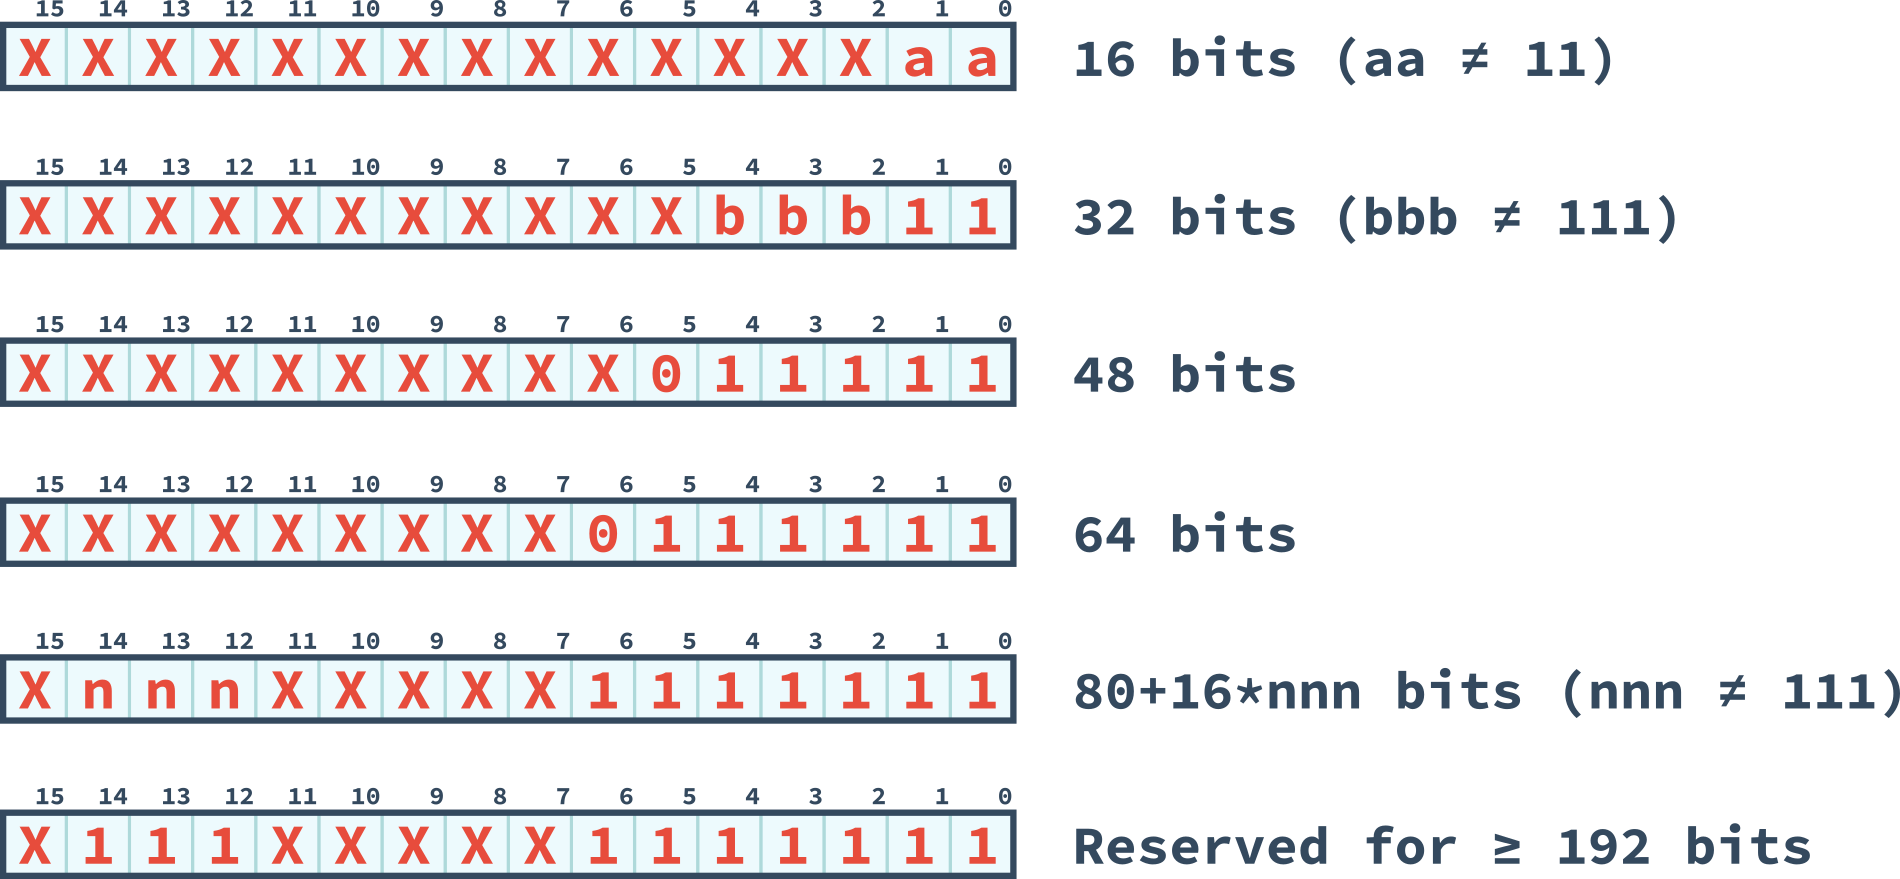
\includegraphics[width=.8\linewidth]
    {../images/instructions/rv_encoding.png}
    \caption{Codificação de instruções de tamanho variável da arquitetura
                \textit{RISC-V}}\label{fig:riscv_var_length}
\end{figure}


    \subsection{Extensão de Registradores de Controle e Estado}
    { A extensão \textbf{Zicsr} implementa o banco de \textit{Control and
        Status Registers} (\textit{CSRs}) e as instruções para acessá-los.
        Esses registradores contemplam um relógio de tempo real (\textit{RTC}),
        contadores de instruções processadas e \textit{ticks} do \textit{clock},
        além de habilitar/desabilitar funcionalidades do processador e checar
        seu estado.
    }

    \subsection{Extensão de Multiplicação e Divisão}
    { As operações aritméticas de multiplicação, divisão e resto de números
        inteiros são implementadas pela extensão \textbf{M}.
    }

    \subsection{Extensões de Ponto Flutuante}
    { A extensão \textbf{F} implementa instruções de ponto flutuante
        \textit{IEEE 754 - 2008} de precisão simples que adiciona
        no processador um banco de 32 registradores de 32 \textit{bits}
        usado para suas operações e um \textit{CSR} para controlar o modo
        de arredondamento e identificar anormalidades na execução de uma
        instrução e.g. divisão por zero.
    }

    { Suas instruções contemplam \textit{load/store} no banco de registradores
        de ponto flutuante, transferência de dados entre os registradores de
        ponto flutuante e os de números inteiros (com ou sem conversão para
        inteiro), operações aritméticas e comparações.
    }

    { A extensão \textbf{D} requer a implementação da extensão \textbf{F} e
        adiciona suporte para operações de ponto flutuante de precisão dupla,
        aumentando a largura do banco de registradores de ponto flutuante
        para 64 \textit{bits}. Há ainda a extensão \textbf{Q} para operações
        de ponto flutuante com precisão quádrupla, que depende da extensão
        \textbf{D} estar implementada e extende a largura do banco de
        registradores de ponto flutuante para 128 \textit{bits}.
    }

    \subsection{Extensões A e Zifencei}
    { A extensão \textbf{A} implementa instruções de acesso atômico a memória,
        enquanto a extensão \textbf{Zifencei} implementa \textit{fencing}
        para escrita e leitura da memória de instruções em um \textit{hart}.
    }

    \subsection{Nomenclatura da implementação}
    { A nomenclatura de um processador \textit{RISC-V} segue a seguinte
        estrutura: as letras \textbf{RV} seguidas da largura do banco de
        registradores (\textbf{32/64}), da letra do módulo base (\textbf{I/E}),
        conforme visto na Seção~\ref{riscv_basic_arch}, e em seguida as outras
        extensões implementadas.
    }

    { As extensões \textbf{M}, \textbf{A}, \textbf{F}, \textbf{D},
        \textbf{Zicsr} e \textbf{Zifencei} utilizadas com o módulo \textbf{I}
        constituem um conjunto considerado um alvo razoável para o
        desenvolvimento de um processador de uso geral. Pela convenção de
        nomenclatura, um processador de 64 \textit{bits} com essa implementação
        se chamaria \textbf{RV64IMAFDZicsr\_Zifencei}. Para uma melhor
        apresentação, o conjunto \textbf{IMAFDZicsr\_Zifencei} pode ser abreviado
        para \textbf{G} (de \textit{\textbf{G}eneral-purpose}). Assim, o
        processador descrito pode ser chaamdo de \textbf{RV64G}.
    }

    \subsection{Outras Extensões}
    { Existem propostas de adição de algumas extensões na especificação da
        \textit{ISA}, como a \textbf{B} para manipulação de \textit{\textbf{B}its}
        e a \textbf{V} para operar \textbf{V}etores, mas ainda não foram
        ratificadas.
    }

    {Há também a possibilidade de se desenvolver extensões próprias. A regra
        de nomenclatura para esse caso é iniciar o nome da extensão com um
        \textbf{X} seguido por um nome alfabético e.g. \textbf{Xhwacha}.
    }

    \subsection{Arquitetura Privilegiada}
    { Para a \textit{ISA RISC-V}, existem quatro níveis de privilégio de acesso,
        sendo eles: o de máquina (nível \textit{bare-metal} que em implementações
        mais simples trata \textit{syscalls}), o de usuário (o nível onde a
        aplicação do usuário é executada), o de supervisor (nível do sistema
        operacional) e o de hipervisor (virtualização).
    }

    { O nível privilegiado de máquina adiciona alguns \textit{CSRs} importantes
        como o \texttt{misa} (\textit{Machine ISA register}), que indica as
        capacidades do processador como largura dos registradores e extensões
        implementadas codificados em \textit{bit fields}, o \texttt{mstatus}
        que controla o estado operacional do \textit{hart} como a habilitação
        de interrupções, o \texttt{mtvec} que contém o endereço de memória
        do tratamento de \textit{traps}, o \texttt{mepc} que guarda o endereço
        de memória onde uma instrução causou uma exceção e o \texttt{mcause}
        que indica a causa da exceção.
    }

    \subsection{Formatos de Instruções}
    { As instruções da arquitetura podem ser separadas em subgrupos de acordo com
        os operadores necessários para o processador interpretá-la. A
        Figura~\ref{fig:riscv_formats} apresenta os formatos das instruções do
        módulo I da \textit{ISA RISC-V}, e, para efeitos de comparação, a
        Figura~\ref{fig:mips_formats} mostra os formatos de instruções equivalentes
        na arquitetura \textit{MIPS32}.
    }

    { Apesar dos formatos das instruções da \textit{RISC-V} serem mais
        complicados que os da \textit{MIPS32} do ponto de vista de um
        humano, para uma máquina eles são muito mais eficientes. Os campos
        do \texttt{opcode}, do \texttt{funct3}, dos registradores \texttt{rs1},
        \texttt{rs2} e \texttt{rd}, e alguns bits dos imediatos \texttt{imm}
        sempre se encontram na mesma posição na instrução. Isso reduz a
        complexidade dos multiplexadores de geração de imediatos e da lógica
        de decodificação da instrução. Além disso, por utilizar imediatos de
        12 \textit{bits} (ou 20 no caso das instruções do tipo \textbf{U})
        em vez de imediatos de 16 \textit{bits} (ou 28 nas instruções do
        tipo \textbf{J}), a \textit{ISA RISC-V} possui mais \textit{bits}
        disponíveis para codificar mais instruções.
    }

    \begin{figure}[H]
    \centering
        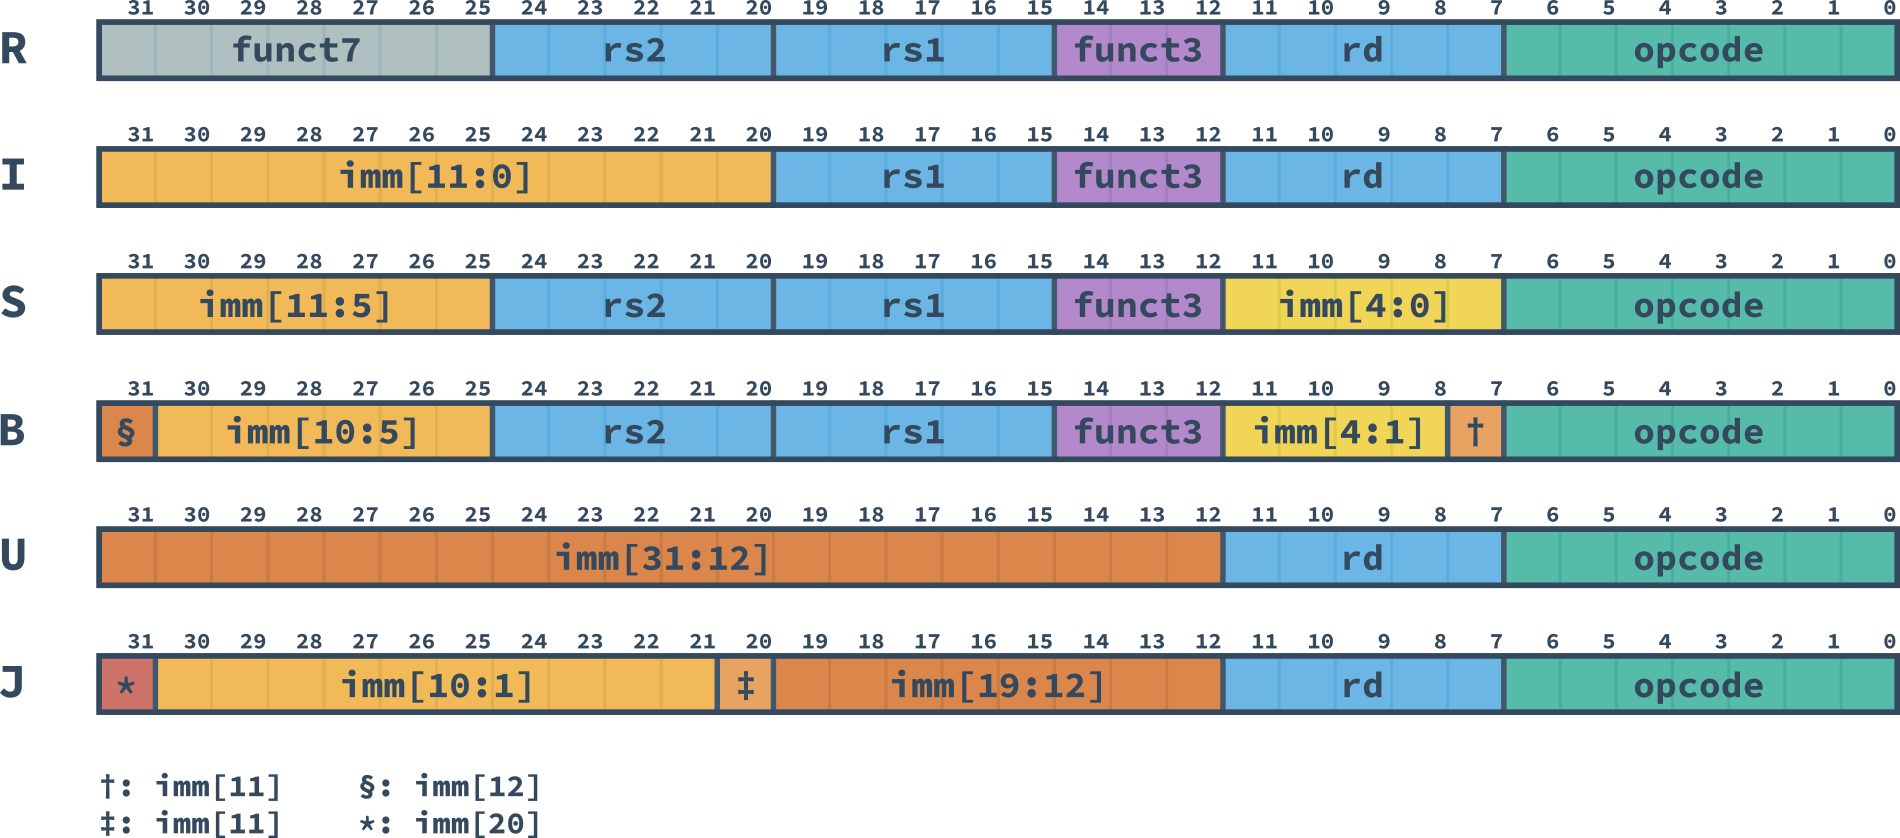
\includegraphics[width=.9\linewidth]
        {../images/instructions/rv32_instructions.png}
        \caption{Formatos de Instruções da \textit{ISA RISC-V}}\label{fig:riscv_formats}
    \end{figure}

    \begin{figure}[H]
    \centering
        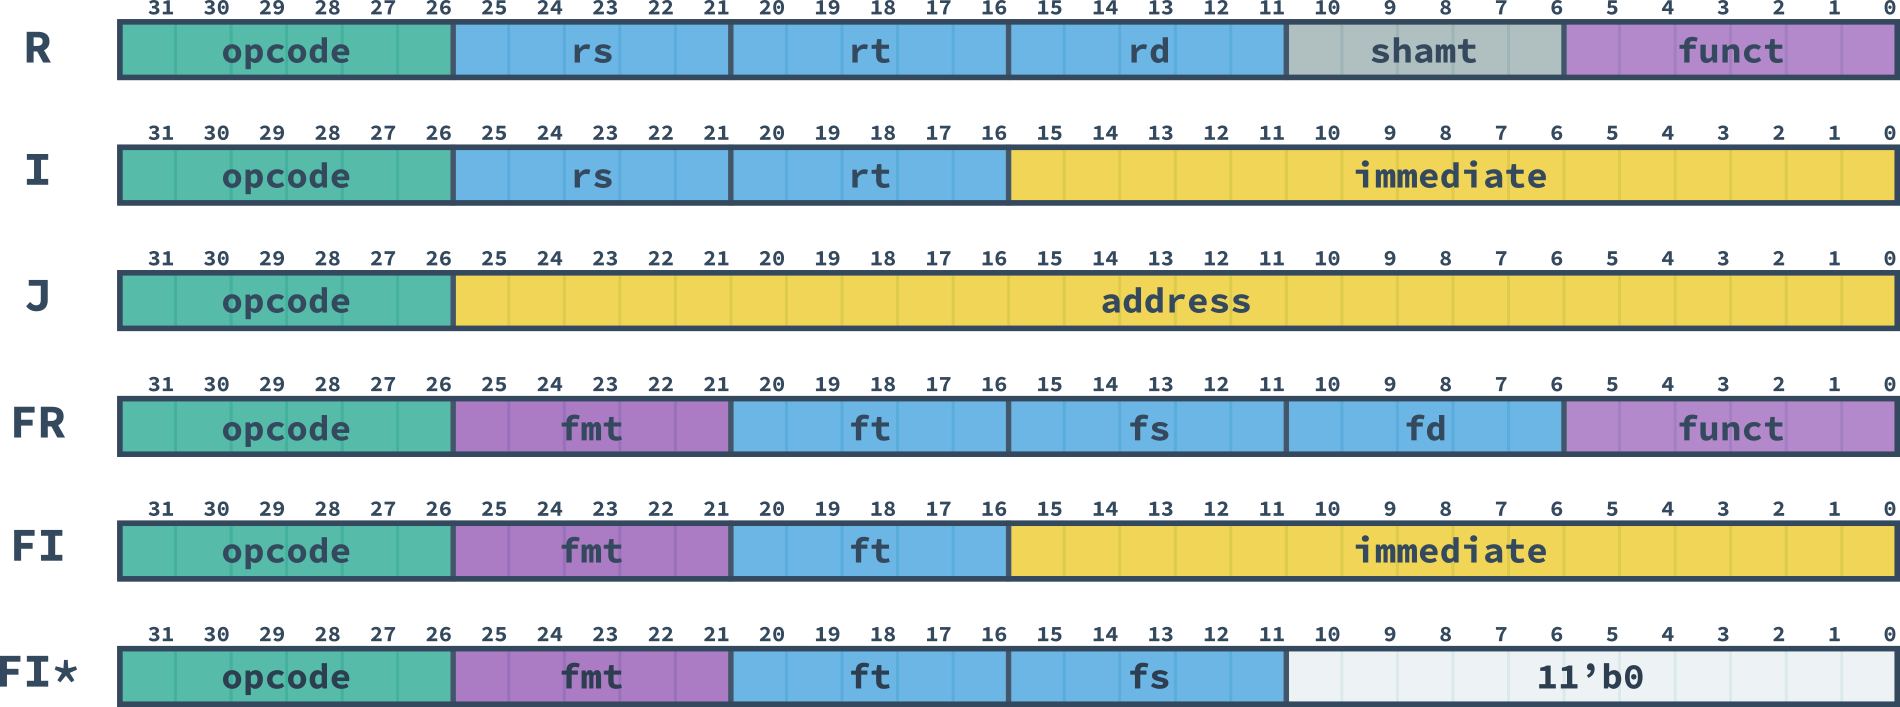
\includegraphics[width=.9\linewidth]
        {../images/instructions/mips32_formats.png}
        \caption{Formatos de Instruções da \textit{ISA MIPS32}}\label{fig:mips_formats}
    \end{figure}

    \subsection{Formatos de Imediatos}
    { Os imediatos são operandos descritos na própria instrução em vez de
        estarem contidos em um registrador. Como os operandos necessitam ter
        a mesma largura que o banco de registradores, algumas regras são
        utilizadas para gerar os imediatos. As figuras a seguir mostram a
        formação de cada tipo de imediato dos formatos das instruções
        apresentadas na Figura~\ref{fig:riscv_formats}.
    }

    \begin{figure}[H]
    \centering
        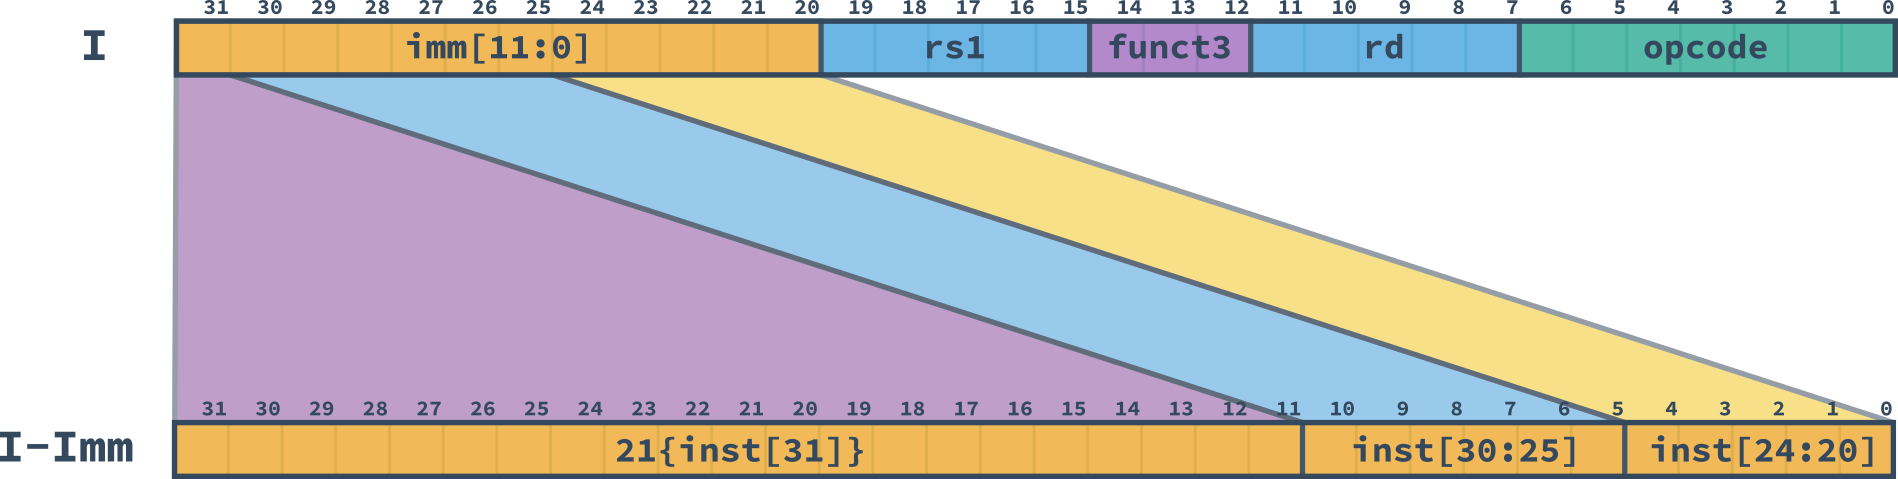
\includegraphics[width=.9\linewidth]
        {../images/instructions/rv32_i_immediate.png}
        \caption{Formação do Imediato de tipo I}\label{fig:riscv_i_imm}
    \end{figure}

    \begin{figure}[H]
    \centering
        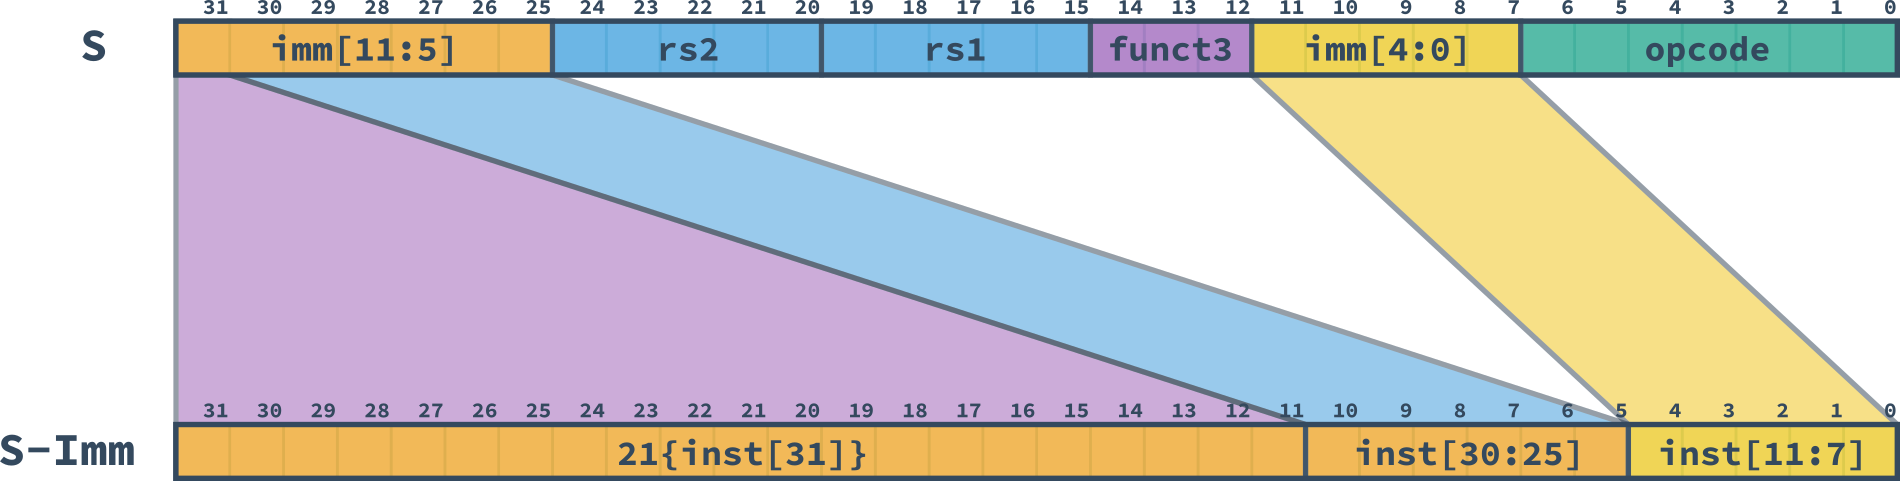
\includegraphics[width=.9\linewidth]
        {../images/instructions/rv32_s_immediate.png}
        \caption{Formação do Imediato de tipo S}\label{fig:riscv_s_imm}
    \end{figure}

    \begin{figure}[H]
    \centering
        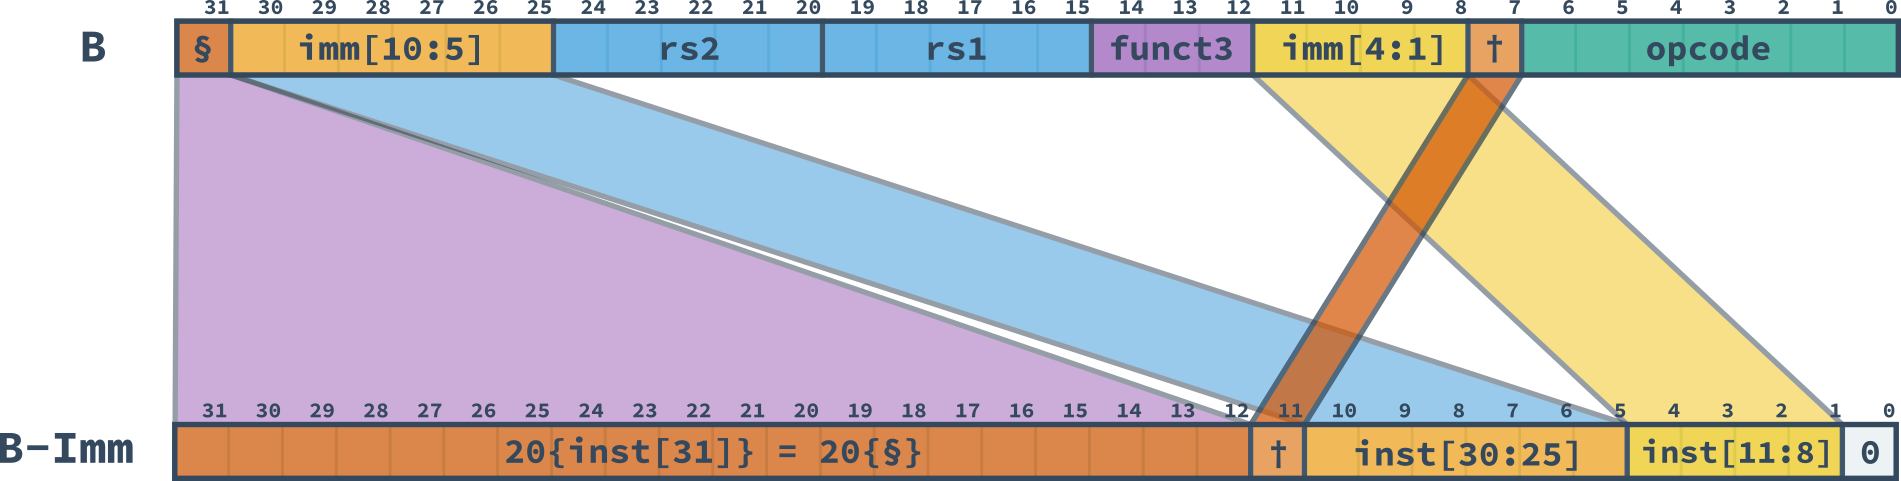
\includegraphics[width=.9\linewidth]
        {../images/instructions/rv32_b_immediate.png}
        \caption{Formação do Imediato de tipo B}\label{fig:riscv_b_imm}
    \end{figure}

    \begin{figure}[H]
    \centering
        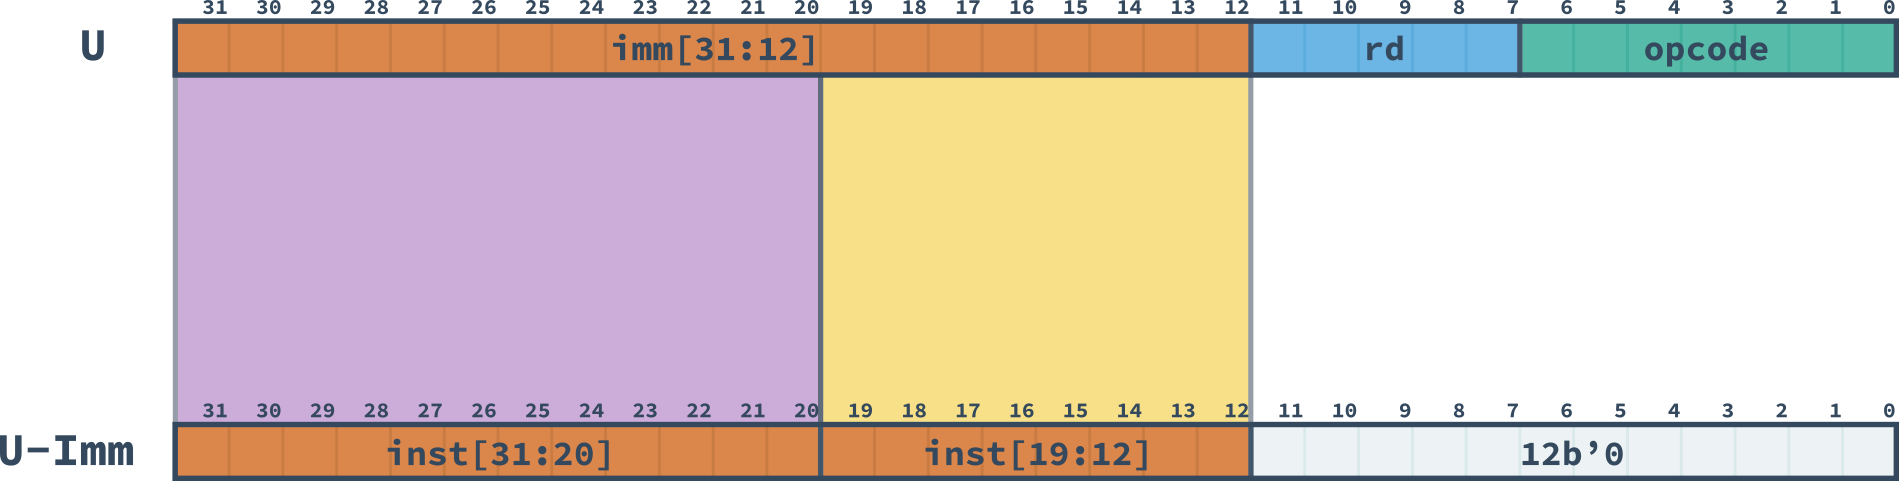
\includegraphics[width=.9\linewidth]
        {../images/instructions/rv32_u_immediate.png}
        \caption{Formação do Imediato de tipo U}\label{fig:riscv_u_imm}
    \end{figure}

    \begin{figure}[H]
    \centering
        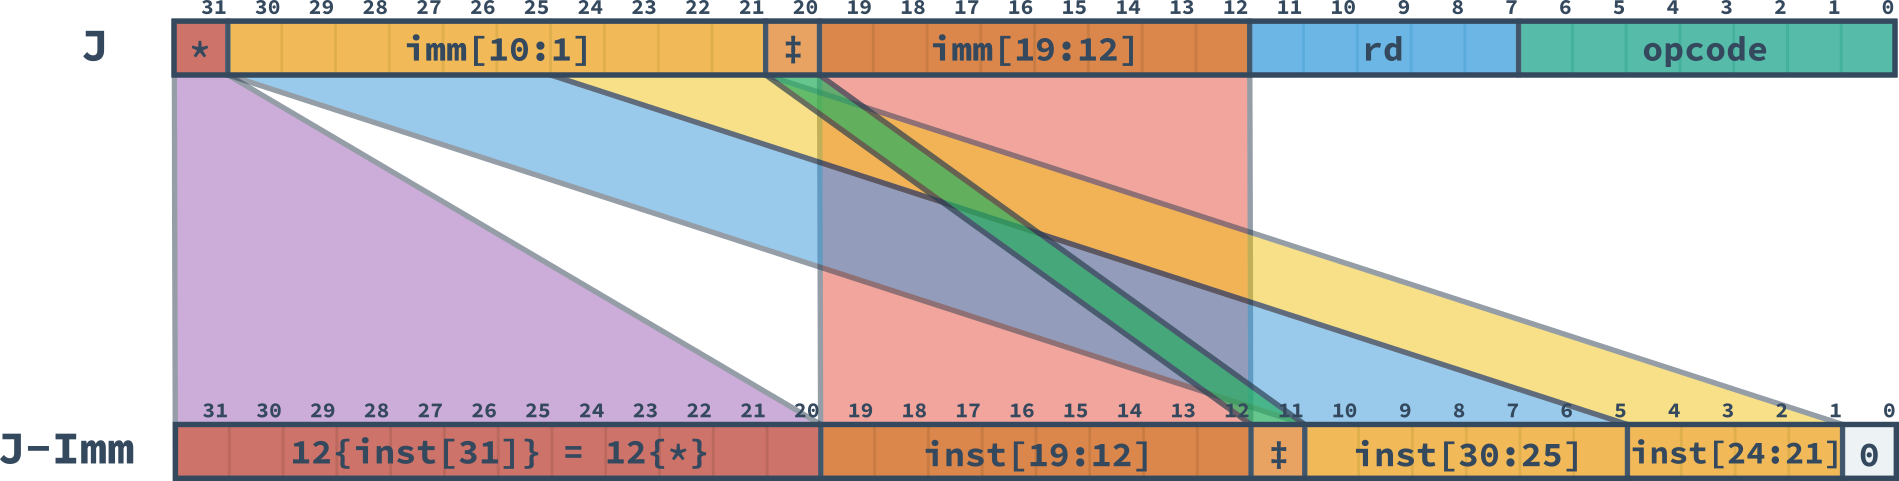
\includegraphics[width=.9\linewidth]
        {../images/instructions/rv32_j_immediate.png}
        \caption{Formação do Imediato de tipo J}\label{fig:riscv_j_imm}
    \end{figure}


\section{\textit{IDE RARS}}\label{rars_cap2}
{ O Ambiente Integrado de Desenvolvimento (\textit{IDE}) \textit{RARS}
    (\textit{RISC-V Assembler and Runtime Simulator}) é um \textit{software
    open source}~\cite{rars_git} utilizado para desenvolver, montar, simular e
    exportar código em \textit{assembly RISC-V}. O projeto é um \textit{fork}
    do \textit{MARS} (\textit{MIPS Assembler and Runtime Simulator}), outro
    \textit{software open source}~\cite{mars_site} muito utilizado em cursos
    de arquitetura de computadores ministrados em \textit{MIPS32}.
}
\begin{figure}[H]
\centering
    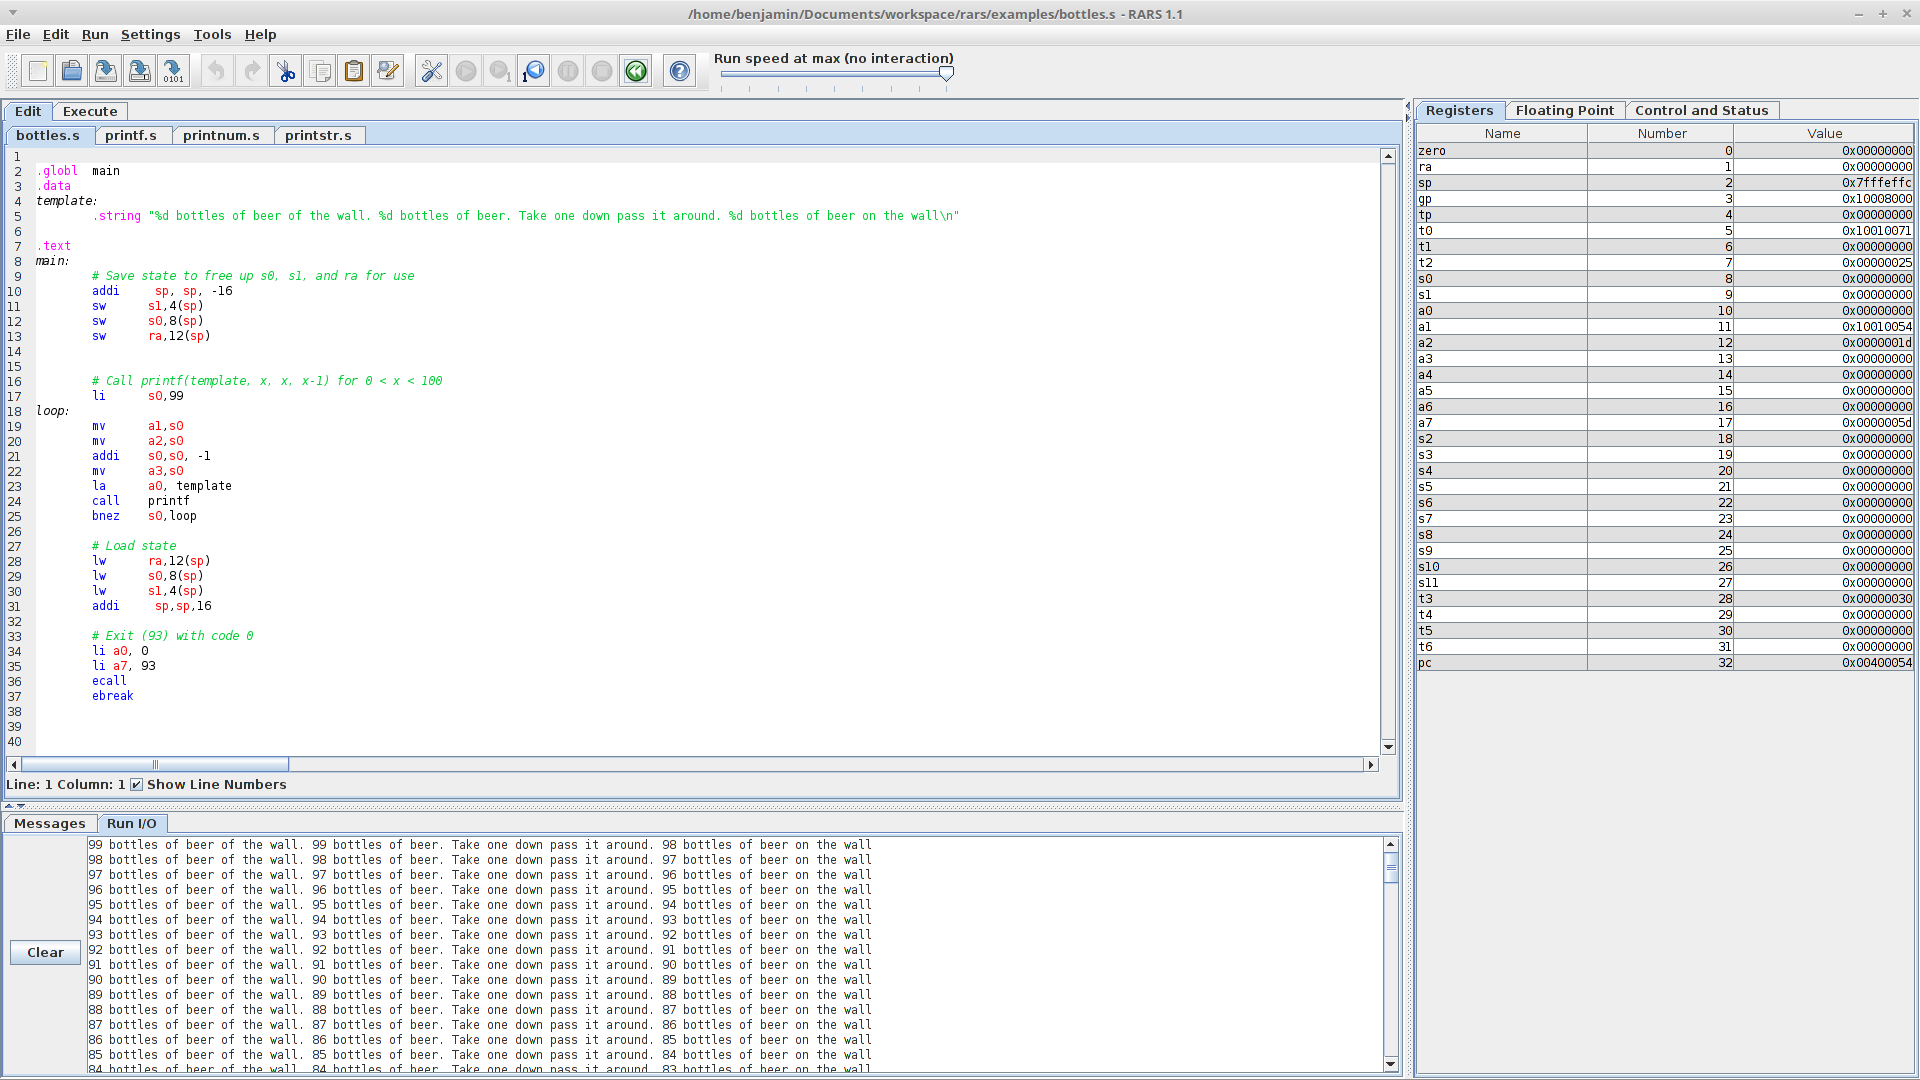
\includegraphics[width=.9\linewidth]{../images/rars.png}
    \caption{\textit{IDE RARS}}\label{fig:rars}
\end{figure}

{ O \textit{RARS} é compatível com as \textit{ISAs} \textbf{RV32IMFD} e
    \textbf{RV64IMFD} com suporte a interrupções e implementa parcialmente a
    extensão \textbf{Zicsr}. Também tem suporte a \textit{syscalls}. Possui
    também um guia de programação em \textit{assembly RISC-V} e pode ser
    utilizado como referência de instruções e pseudo-instruções.
}

{ Com sua função de simulador, permite executar o código instrução por instrução,
    mostrando as modificações nos bancos de registradores e na memória. Além
    disso, permite exportar o programa montado no formato \textit{.mif} para
    uso na inicialização de memória de \textit{FPGAs}.
}


\section{Microarquiteturas}
{ Enquanto o campo de arquitetura de computadores explora a especificação dos
    conjuntos de instruções, a organização de computadores trata da forma com que
    as especificações são implementadas. Os padrões de implementação de
    \textit{ISAs} são chamados de microarquiteturas, e esses padrões podem ser
    combinados para produzir soluções mais complexas.
}

{ Processadores são circuitos elétricos, e podem ser descritos por diagramas.
    Nesses diagramas, o caminho de dados (\textit{datapath}) representa a
    conexão feita entre blocos lógicos por barramentos onde os sinais a serem
    processados trafegam. A unidade de controle é responsável por interpretar as
    instruções recebidas e comandar os blocos lógicos para executar o comando.
    Os blocos lógicos são as Unidades de Lógica e Aritmética (ULA, ou
    \textit{ALU} em inglês), bancos de registradores (\textit{regfiles})
    multiplexadores e blocos de memória.
}

    \subsection{Uniciclo}
    { Processadores uniciclo são implementados de forma com que cada instrução
        seja recuperada (\textit{fetch}), decodificada (\textit{decode}),
        executada e finalizada (\textit{retire}) durante um único \textit{tick}
        do \textit{clock}. Para isso, a unidade de controle deve conter somente
        lógica combinacional e a frequência de operação do \textit{clock} deve
        ser projetada para o pior caso, ou seja, a instrução que leva mais tempo
        entre seu \textit{fetching} e seu \textit{retiring}.
    }

    { A implementação da microarquitetura uniciclo é uma das mais mais simples
        de se fazer, mas o processador resultante apresenta baixa frequência de
        processamento. Para \textit{workloads} que utilizam muitas instruções
        complexas, seu desempenho pode ser parecido ou até melhor que implementações
        mais elaboradas, mas se a maioria da carga de processamento for de
        instruções rápidas, o uniciclo sofre uma penalidade por ficar ocioso
        durante parte do seu ciclo.
    }

    \subsection{Multiciclo}
    { A microarquitetura multiciclo também é conhecida como implementação por
        microcódigo. As instruções são ``quebradas'' em etapas menores, como
        o acesso à memória, a leitura do banco de registradores, a seleção de um
        sinal multiplexado, a realização de uma operação lógica ou aritmética,
        dentre outras possibilidades. A unidade de controle é implementada por
        lógica sequencial como uma máquina de estados finitos, e a frequência
        máxima de operação é limitada pela etapa mais lenta da máquina de estados.
    }

    { Como a quantidade de estados que uma instrução deve passar entre seu
        \textit{fetching} e \textit{retiring} depende de sua complexidade e de
        como a máquina de estados foi projetada, a frequência do \textit{clock}
        costuma ser mais alta que de uma implementação uniciclo, mas isso não
        significa que seu desempenho será melhor, pois o desempenho também depende
        do \textit{workload}. Se a maioria das instruções executadas precisa
        passar por diversos estados para serem completadas, o somatório de ciclos
        menores pode resultar em um intervalo de tempo maior que o do ciclo único.
    }

    \subsection{\textit{Pipeline}}\label{cap2_fwd_hzd}
    { Uma implementação \textit{pipeline} consiste em inserir registradores entre
        os blocos lógicos do \textit{datapath}, o dividindo em etapas. O objetivo
        é ser capaz de processar mais de uma instrução por vez. A
        Figura~\ref{fig:pipe_generic} mostra um \textit{pipeline} genérico de
        quatro estágios. O processo inicia com o \textit{fetching} de uma instrução
        no primeiro ciclo do \textit{clock}. No segundo ciclo do \textit{clock},
        a primeira instrução passa para o estágio de \textit{decode} e uma nova
        instrução entra no primeiro estágio do \textit{pipeline}. No terceiro
        \textit{tick}, a primeira instrução está no terceiro estágio, a segunda
        no segundo estágio e a terceira no primeiro estágio. No quarto ciclo,
        a primeira instrução está no quarto estágio, a segunda instrução no
        terceiro estágio, a terceira instrução no segundo estágio e a quarta
        instrução acaba de entrar no \textit{pipeline}. No ciclo seguinte, a
        primeira instrução é finalizada, as outras três instruções passam para
        o estágio seguinte e uma nova instrução entra no primeiro estágio do
        \textit{pipeline}.
    }

    \begin{figure}[H]
    \centering
        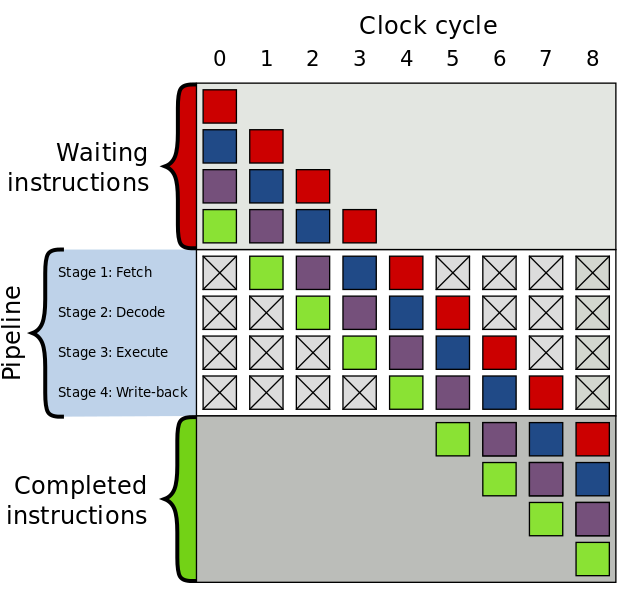
\includegraphics[width=.65\linewidth]{../images/pipeline_4_stage.png}
        \caption[\textit{Pipeline} genérico com 4 estágios]{\textit{Pipeline}
            genérico com 4 estágios. \quad Fonte:~\cite{pipe_generic}}\label{fig:pipe_generic}
    \end{figure}

    { A frequência do \textit{clock} é limitada pelo estágio mais lento. O objetivo
        é manter o \textit{pipeline} com todos os seus estágios preenchidos, e
        assim, a cada \textit{tick}, uma instrução é completada, sendo uma
        implementação com ótimo desempenho. Porém, é comum que uma instrução
        precise do resultado de outra instrução que ainda não foi finalizada.
    }

    { Uma solução simples porém ineficiente para o problema é limpar os estágios
        anteriores, inserindo \texttt{nop}s (instruções que não realizam nenhuma
        tarefa) até que o resultado esteja disponível e voltar a preencher o
        \textit{pipeline}. Uma solução mais robusta seria implementar uma
        unidade de identificação e tratamento de \textit{forwards} e \textit{hazards}.
        \textit{Forwards} ocorrem quando a instrução anterior ainda não finalizou,
        mas seu resultado já está disponível em algum estágio do \textit{pipeline}
        e o valor pode ser injetado na etapa que precisa dele. Já os \textit{hazards}
        são situações onde o \textit{forward} não é possível e \texttt{nop}s
        precisam ser inseridos.
    }


\section{Representação de \textit{Hardware}}
{ Existem diversas maneiras de representar circuitos eletrônicos. Na programação
    visual, as entradas e saídas dos blocos funcionais são conectados de forma
    gráfica, montando um diagrama do circuito. Já as linguagens de descrição de
    \textit{hardware} (\textit{HDLs}) como o \textit{Verilog} e o \textit{VHDL}
    permitem uma descrição precisa da estrutura e comportamento dos circuitos.
    Outra forma de representação utiliza a síntese de alto nível (\textit{High-Level Synthesis}),
    onde se desenvolve um algoritmo em linguagens como \textit{C++} ou \textit{MATLAB},
    que será ``traduzido'' para um circuito eletrônico.
}

{ Essas reprentações permitem a geração de \textit{netlists} utilizadas para
    simular o projeto, sintetizá-lo em \textit{FPGAs} ou fazer o \textit{tapeout}
    para produção de \textit{chips}.
}

    \subsection{\textit{Verilog}}
    { \textit{Verilog} é uma \textit{HDL} comumente utilizada no projeto \textit{RTL}
        de circuitos lógicos. Módulos escritos em \textit{Verilog} descrevem seus
        sinais de entrada e saída como parâmetros para a conexão com outros módulos.
        As suas principais ``variáveis'' são \textit{wires} (fios que conectam
        um sinal a outro) e \textit{regs} (registradores ou \textit{drivers} de
        sinal). A lógica do módulo pode ser implementada por \textit{assignments}
        (a conexão de um fio a um registrador ou um \textit{driver}) ou por
        blocos de lógica sequencial ou combinacional, usando operadores blocantes
        (\texttt{=}) ou não-blocantes (\texttt{<=}).
    }

    { Para quem está acostumado com linguagens imperativas como o \textit{C},
        há uma barreira inicial para entender que o código não é executado linha
        por linha, mas sim de maneira concorrente, e que a escolha entre operadores
        blocantes e não-blocantes afeta a forma com que os sinais são propagados
        no circuito.
    }

    { A sintaxe do \textit{Verilog} é menos verbosa que a do \textit{VHDL}, que
        é fortemente tipada. Enquanto a verificação formal de \textit{designs}
        em \textit{VHDL} é um processo mais natural, o \textit{Verilog} possui
        uma curva de aprendizado menor, sendo ideal para o primeiro contato com
        linguagens de descrição de \textit{hardware}.
    }

    \subsection{Análise e Síntese}
    { O processo de análise de representações de \textit{hardware} verifica a
        sintaxe da representação, identificando estruturas inválidas, sinais não
        conectados e possíveis erros semânticos que farão com que a \textit{netlist}
        não possa ser gerada ou não se comporte conforme o esperado.
    }

    { Já a síntese é o processo de transformar a estrutura analisada em uma
        \textit{netlist}, estrutura que contém a lista de componentes eletrônicos
        do \textit{design} e a descrição de como eles se conectam.
    }

    \subsection{\textit{Fitting} e \textit{Timing Analyzer}}
    { O \textit{fitting} é o processo de criar as rotas de conexão da \textit{netlist}.
        O \textit{design} é mapeado para a plataforma onde será implementado.
        Já o \textit{timing analyzer} define restrições de temporização entre
        elementos do circuito que o \textit{fitter} tenta respeitar. O
        \textit{fitter} itera diversas vezes o posicionamento e roteamento dos
        componentes até gerar o resultado final.
    }

    { Com a \textit{netlist} roteada, o \textit{Timing Analyzer} é executado
        novamente, testa se o \textit{fitter} conseguiu atender às restrições e
        gera um relatório. Caso alguma rstrição essencial não for respeitada,
        o \textit{Fitter} pode ser novamente executado com opções diferentes que
        impactarão outras características do circuito final, como quantidade de
        componentes e consumo energético.
    }

    { Pode ser necessário reimplementar a
        representação do \textit{hardware} para que todos os requisitos de projeto
        sejam atendidos.
    }


\section{Field Programmable Gate Arrays}
{ \textit{Field Programmable Gate Arrays} (\textit{FPGAs}) são circuitos
    integrados que permitem o desenvolvimento de circuitos lógicos
    reconfiguráveis. Por serem reprogramáveis, as \textit{FPGAs} geram uma
    grande economia em tempo de desenvolvimento e em custos como os de
    prototipagem, validação e manufatura do projeto em relação aos circuitos de
    aplicações específicas, os \textit{ASICs}, e aos projetos
    \textit{full-custom}. As \textit{FPGAs} podem ser tanto o passo
    intermediário no projeto de um \textit{ASIC} ou \textit{full-custom} quanto
    o meio final do projeto quando a reconfigurabilidade e os preços muito mais
    acessíveis forem fatores importantes.
}

{ Cada fabricante de \textit{FPGAs} possui seu \textit{software} de
    desenvolvimento, ou \textit{SDKs}. A indústria de \textit{hardware} é
    extremamente protecionista com sua propriedade intelectual (tanto que os
    \textit{designs} de módulos ou circuitos completos são chamados de \textit{IPs},
    termo derivado de \textit{\textbf{I}ntellectual \textbf{P}roperty}), sendo
    a maioria dessas ferramentas de código proprietário. Para a Intel Altera,
    essa plataforma é o Quartus Prime.
}

{ \textit{FPGAs} mais modernas possuem, além do arranjo de portas lógicas,
    blocos de memória, \textit{Phase-Locked Loops} (\textit{PLLs}),
    \textit{Digital Signal Processors} (\textit{DSPs}) e \textit{System on
    Chips} (\textit{SoCs}). Os blocos de memória internos funcionam como a memória
    \textit{cache} de um microprocessador, armazenando os dados próximo ao seu
    local de processamento para diminuir a latência. Os \textit{PLLs} permitem criar
    sinais de \textit{clock} com diversas frequências a partir de um relógio de
    referência, e podem ser reconfigurados a tempo de execução. \textit{DSPs}
    são responsáveis pelo processamento de sinais analógicos discretizados, e
    podem ser utilizados como multiplicadores de baixa latência. Já os
    \textit{SoCs} são microprocessadores como os ARM presentes em celulares,
    e são capazes de executar sistemas operacionais como o Linux.
}

{ Além de disponíveis na forma de \textit{chips} para a integração com placas
    de circuito impresso customizadas (\textit{PCBs}), as \textit{FPGAs} possuem
    \textit{kits} de desenvolvimento com diversos periféricos para auxiliar no
    processo de criação de soluções. Esses \textit{kits} são a principal ferramenta
    de aprendizagem no universo dos circuitos reconfiguráveis. No Laboratório de
    Informática da UnB, as placas \textit{terasIC DE1-SoC} com a \textit{FPGA
    Intel Cyclone V SoC} estão disponíveis para os alunos de OAC desenvolverem
    seus projetos.
}

    \subsection{Arquitetura Generalizada de uma FPGA}
    { De forma genérica, uma \textit{FPGA} possui blocos lógicos, chaves de
        interconexão, blocos de conexão direta e portas de entrada e saída,
        conforme apresentado na Figura~\ref{fig:fpga_general_arch}.
    }

    \begin{figure}[H]
    \centering
    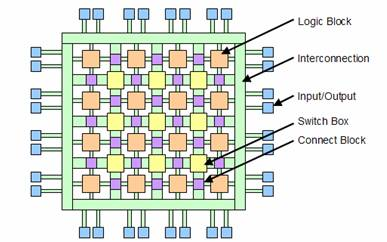
\includegraphics[width=.7\linewidth]
        {../images/fpga_architecture_abstraction_-_olin_college.jpg}
        \caption[Abstração da arquitetura de uma FPGA]
            {Abstração da arquitetura de uma FPGA.\quad Fonte:~\cite{fpga_arch_abstraction}}
        \label{fig:fpga_general_arch}
    \end{figure}

    { Os blocos lógicos possuem \textit{lookup tables}, registradores, somadores
        e multiplexadores. É neles que a lógica reconfigurável é implementada.
        Já as chaves de interconexão são responsáveis por conectar os diversos
        blocos lógicos da \textit{FPGA}. A Figura~\ref{fig:fpga_switch_box} exemplifica
        como é feito o roteamento da malha de interconexão. Os blocos de conexão
        direta são um tipo especial de chave de interconexão, e sua função é ligar
        blocos lógicos adjacentes. Por fim, as portas de entrada e saída conectam
        a \textit{FPGA} ao ``mundo externo'' e.g. \textit{drivers} de áudio e vídeo.
    }

    \begin{figure}[H]
    \centering
    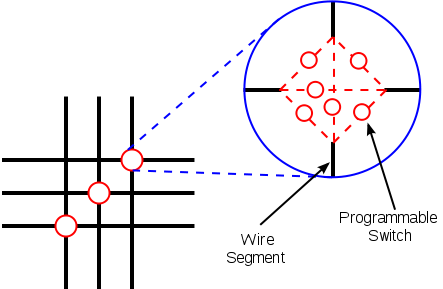
\includegraphics[width=.5\linewidth]
        {../images/switch_box_wikimedia.png}
        \caption[Funcionamento da chave de interconexão]
            {Funcionamento da chave de interconexão.\quad Fonte:~\cite{fpga_switch_box}}
        \label{fig:fpga_switch_box}
    \end{figure}


    \subsection{Arquitetura da FPGA Cyclone V SoC}
    { A Figura~\ref{fig:cyclone_v_arch} apresenta a arquitetura da
        \textit{FPGA Cyclone V SoC}. O \textit{chip} possui um processador
        \textit{ARM} integrado, blocos de memória embutidos, \textit{DSPs} para
        acelerar operações como multiplicação de números ou processamento de
        sinais genéricos, diversos pinos para integrar o \textit{chip} a
        um projeto de circuito mais complexo, \textit{PLLs} para gerar diversos
        sinais de \textit{clock}, entre outras funcionalidades.
    }

    \begin{figure}[H]
    \centering
    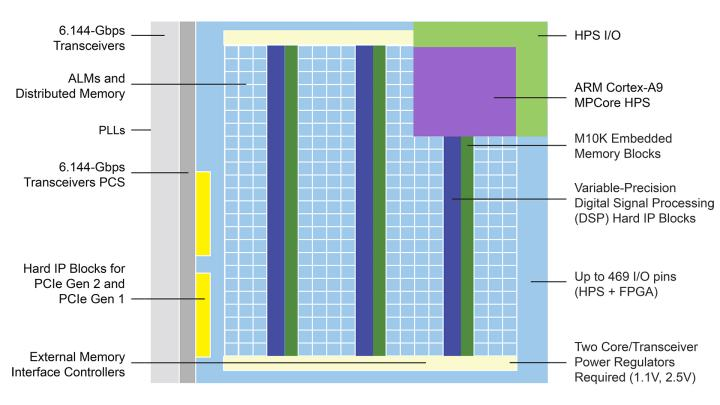
\includegraphics[width=1\linewidth]
        {../images/altera_cyclone_v_soc_architectural_downscale.jpg}
        \caption[Arquitetura da FPGA Intel Cyclone V SoC]
            {Arquitetura da \textit{FPGA Altera Cyclone V SoC}.\quad Fonte:~\cite{cyclone_v_soc}}
        \label{fig:cyclone_v_arch}
    \end{figure}

        \subsubsection{Adaptative Logic Modules}
        { Os blocos lógicos, como mostrados na abstração da Figura~\ref{fig:fpga_general_arch}
            são implementados na \textit{FPGA Cyclone V SoC} como
            \textit{Adaptative Logic Modules}, conforme a Figura~\ref{fig:fpga_alm}.
            Como os \textit{ALMs} são blocos genéricos, há um \textit{trade-off}
            entre configurabilidade e performance.
        }

        \begin{figure}[H]
        \centering
        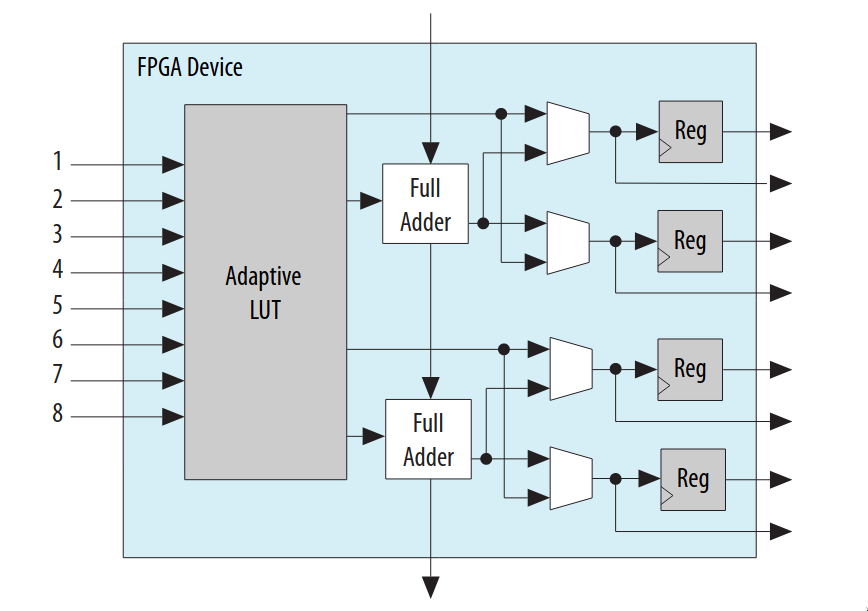
\includegraphics[width=.7\linewidth]
            {../images/intel_alm_high_level.png}
            \caption[Diagrama de blocos de um ALM]
                {Diagrama de blocos de um ALM.\quad Fonte:~\cite{cyclone_alm}}
            \label{fig:fpga_alm}
        \end{figure}


        \subsubsection{Embedded Memory Blocks}
        { Como mostrado na Figura~\ref{fig:cyclone_v_arch}, existem blocos de
            memória embutidos na \textit{FPGA}. Esses blocos são o equivalente
            a uma memória \textit{cache L1}, sendo a camada de memória mais próxima
            dos registradores. Para utilizá-los no \textit{design} do circuito,
            blocos do \textit{IP} de memória são configurados e instanciados
            pelo programa de desenvolvimento para gerar um módulo integrável no
            resto do \textit{design}.
        }

        { As placas de desenvolvimento podem possuir outros tipos de memória,
            como as \textit{SRAM} e \textit{DRAM}. Apesar de possuírem capacidade
            de armazenamento bem maiores que os blocos embutidos, seus
            módulos controladores são mais complexos e apresentam latência maior
            para leitura e escrita de dados. Para seu uso eficiente, é necessário
            implementar camadas de \textit{caching} para que as operações de
            \textit{input} e \textit{output} (\textit{IO}) não se tornem um
            gargalo que comprometa o resto do \textit{design}.
        }


\section{Estado da Arte dos processadores RISC-V}
{ Por alguns anos, processadores com arquitetura \textit{RISC-V} só podiam
    ser utilizados por meio de emuladores como o \textit{qemu}~\cite{qemu_riscv}
    ou em \textit{FPGAs}. Diversos \textit{soft-cores} \textit{open source},
    tanto experimentais (como o desenvolvido neste trabalho) quanto de alto
    desempenho podem ser encontrados na \textit{internet} e utilizados por
    qualquer pessoa interessada. Um dos processadores alto desempenho disponíveis
    é o \textit{BOOM}~\cite{boom_berkeley}, processador com execução
    \textit{Out of Order} desenvolvido na universidade americana \textit{UC Berkeley}
    pelo mesmo departamento onde surgiu a arquitetura \textit{RISC-V}, o
    \textit{Berkeley Architecture Research}~\cite{berkeley_bar}. O processador
    pode ser sintetizado em instâncias \textit{EC2 F1} da
    \textit{AWS}~\cite{boom_aws}, eliminando a necessidade de possuir uma
    \textit{FPGA} de alto desempenho para usufruir do projeto.
}

{ Outro projeto \textit{open source} notável é o \textit{Shakti}~\cite{shakti},
    ecossistema desenvolvido na universidade indiana \textit{IIT-Madras} com
    diversas implementações para os mais diversos usos, que variam desde
    microcontroladores de 32 \textit{bits}, superescalares de 64 \textit{bits}
    para aplicação em \textit{desktops} e servidores até processadores de alta
    performance com mais de 32 \textit{cores}~\cite{shakti_types}.
}

{ Porém, a presença apenas de \textit{soft-cores} limita as possíveis aplicações
    da arquitetura. Algumas fabricantes já divulgaram planos para começar a usar
    microcontroladores com a arquitetura em seus produtos, como é o caso dos
    controladores de discos rígidos e \textit{SSDs} da
    \textit{Western Digital}~\cite{western_riscv} e da Nvidia como o substituto
    dos controladores \textit{Falcon} de suas placas de vídeo~\cite{nvidia_riscv}.
    Ainda não se sabe se as empresas já utilizam os controladores em seus
    \textit{hardwares}, se a adoção ainda está em fase de projeto ou se a ideia
    foi abandonada.
}

{ Porém, começam a surgir no mercado microcontroladores e \textit{Single
    Board Computers (SBCs)} com preços acessíveis. Placas como a linha
    \textit{Sipeed} da \textit{Seed} se equiparam aos \textit{MCUs
    ESP32}~\cite{hackaday_sipeed}, e outras como a \textit{SiFive HiFive1}
    se assemelham aos \textit{arduinos}~\cite{hifive_arduino}.
}

{ Há uma expectativa de \textit{SBCs} mais robustos, capazes de rodar um
    sistema operacional de uso geral, como um \textit{Raspberry Pi}. Existem
    alguns pré-lançamentos de placas para atender essa demanda, como a
    \textit{SiFive HiFive Unmatched}~\cite{hifive_unmatched} e a
    \textit{BeagleV}~\cite{beaglev}.
}

{ A empresa \textit{SiFive}, liderada pelos criadores da arquitetura, produzirá
    em parceria com a \textit{TSMC (Taiwan Semiconductor Manufacturing Company)}
    o primeiro processador \textit{RISC-V} de 32 \textit{bits} em tecnologia
    de 5nm~\cite{sifive_tsmc}. A \textit{TSMC} é a \textit{foundry} líder em
    manufatura de circuitos integrados no mundo.
}

{ Atualmente, compilar códigos em \textit{C/C++} para \textit{targets RISC-V}
    não envolve mais a instalação de \textit{toolchains} complicadas e frágeis.
    Tanto o \textit{gcc}~\cite{gcc_riscv} quanto o \textit{clang}~\cite{clang_riscv}
    já oferecem suporte para o \textit{RISC-V}, eliminando assim uma barreira
    para a adoção da arquitetura.
}

{ Uma outra característica essencial para o uso do \textit{RISC-V} em sistemas
    de uso geral é a existência de sistemas operacionais que funcionem na
    plataforma. Desde a versão 4.15, o \textit{kernel} do \textit{linux}
    oferece suporte para a arquitetura~\cite{linux_kernel}. \textit{Distros}
    como \textit{Fedora}~\cite{fedora_experimental},
    e \textit{Alpine}~\cite{alpine_experimental} já possuem suporte experimental.
    A chinesa \textit{Alibaba} fez o \textit{port} do \textit{OS Android}
    para um de seus \textit{SoCs RISC-V}~\cite{alibaba_android}. Alguns
    ecossistemas mais robustos possuem \textit{ports} completos, como é o
    caso do \textit{Haiku-OS}~\cite{haiku_riscv} e do \textit{microkernel
    seL4}~\cite{sel4_riscv}, possibilitando o uso em ambientes industriais
    e áreas que exigem maior robustez do sistema operacional.
}

{ Uma das surpresas na adoção da arquitetura \textit{RISC-V} nos seus
    \textit{designs} veio da \textit{MIPS Technologies}, detentora das
    patentes das arquiteturas \textit{MIPS}. Em 2013, a empresa foi adquirida
    pela \textit{Imagination Technologies}~\cite{imagination_technologies_acq},
    e lançou alguns \textit{development kits} voltados a visão computacional
    e microcontroladores, mas não conseguiu dar tração aos projetos.
    Em 2017 a companhia foi novamente vendida para a \textit{Tailwood
    Venture Capital}~\cite{tailwood_acq}, que tentou capitalizar em cima dos
    \textit{royalties} da arquitetura. Porém, em 2018 a companhia foi vendida
    novamente para a \textit{Wave Computing}~\cite{wave_comp_acq}, companhia
    voltada para aplicações de inteligência artificial. Em 2020, a
    \textit{Wave Computing} declara falência~\cite{wave_comp_bankrupt},
    demitindo todos os seus funcionários. Em março desse ano, a empresa
    conseguiu se recuperar da falência, mudou o nome da companhia para
    \textit{MIPS} e anunciou que seus novos \textit{designs} serão baseados
    na arquitetura \textit{RISC-V}~\cite{mips_reborn}. Atualmente, a empresa
    \textit{MIPS} integra a \textit{RISC-V Foundation} como Membro Estratégico.
}


\section{Observações finais da Revisão Teórica}
{ O capítulo abordou os conceitos que formam o alicerce do trabalho. O capítulo
    seguinte apresentará a proposta do projeto, descrevendo sua implementação
    e documentando o processo de execução e modificação do produto final a fim
    de permitir sua utilização futura.
}

